\documentclass[11pt]{article}
\usepackage[margin=1in]{geometry}
\usepackage{amsmath,amssymb}
\usepackage{graphicx}
\usepackage{hyperref}
\usepackage{enumitem}
\usepackage{booktabs}
\usepackage{float}
\usepackage{algorithm}
\usepackage{algpseudocode}
\usepackage[font=small,labelfont=bf]{caption}

\title{ChemCS: Integrating Constraint Satisfaction and Diffusion\\Models for Chemically Valid Molecular Generation}
\author{Sreepranav Chetlapalli}
\date{}

\begin{document}
\maketitle

% ===================================================================
% ABSTRACT
% ===================================================================
\begin{abstract}
<<<<<<< HEAD
Molecular generation with diffusion models has shown promise for drug
discovery and materials design, yet these models frequently produce
chemically invalid structures---atoms with too many bonds, reactions that
violate mass conservation, or mismatched formal charges. Most existing
approaches address this by filtering invalid outputs \emph{after}
generation is complete, which wastes computation and provides no
mechanism for mid-trajectory correction.

This paper presents \textbf{ChemCS}, a system that integrates a
constraint-satisfaction supervisor directly into the reverse-diffusion
loop of a graph neural network (GNN) molecular generator. At every
denoising step the supervisor decodes the current molecular state,
verifies chemical axioms (valency limits, mass conservation, charge
balance, and atom counts), and either commits the step, applies targeted
repairs, or backtracks to a previously valid state. The constraint
checker uses the \textbf{Z3} SMT solver from Microsoft Research to
formulate and verify chemical rules as satisfiability queries.

The generator itself is a lightweight two-layer GNN that operates on
atom-level feature vectors and an adjacency matrix of bond orders. A
companion PyTorch training pipeline adds differentiable constraint
penalties---for valency and element conservation---to the standard
denoising loss, with a curriculum schedule that ramps these penalties
gradually to avoid destabilizing early training.

On a benchmark of three representative reactions (SN2, combustion,
acid--base) with 50~random seeds each, supervised generation achieves
\textbf{100\% valency validity} compared with roughly \textbf{15\%} for
unsupervised generation with the same untrained network. The project
includes 118~unit tests covering every major component.
=======
Generative models for molecules can produce structures that violate basic chemistry rules such as
bond valency limits, mass conservation, and charge balance. Rather than filtering out bad outputs
after the fact, this work proposes \textbf{ChemCS}, a system that enforces chemical constraints
during the generative process. We pair a small graph neural network (GNN) diffusion model
with a \textbf{supervisor loop} backed by Microsoft's Z3 theorem prover. At each reverse-diffusion 
step, the supervisor checks the candidate molecule against a set of chemical axioms and either 
commits the step, applies a lightweight correction, or backtracks. We also introduce a 
\textbf{constraint-aware training loss} with a curriculum schedule so the
model can learn to avoid violations on its own. Experiments across three reaction types show that
supervised generation achieves 100\% valency validity compared to roughly 15\% for
unsupervised generation with the same random-weight model, and that the training loss drops by
over 30\% within 100 epochs on a small dataset.
>>>>>>> d673a4a1e1a4c808da67c24e5bf79449fd6f4617
\end{abstract}

% ===================================================================
% 1  INTRODUCTION
% ===================================================================
\section{Introduction}

<<<<<<< HEAD
Generating novel molecular structures is a central challenge in
computational chemistry. Applications range from \emph{de novo} drug
design, where candidate molecules must satisfy pharmacological
constraints, to materials science, where target properties such as band
gap or thermal stability guide the search. In recent years
\emph{diffusion models}---originally developed for image
generation---have been adapted to molecular graphs with encouraging
results~\cite{hoogeboom2022equivariant, vignac2023digress}.
=======
Molecular generation is important for drug discovery, materials science, and chemical engineering.
Recent work has applied diffusion models --- originally designed for images --- to molecular graphs,
treating atoms as nodes and bonds as edges. The model starts from noise and iteratively denoises
toward a valid molecule.
>>>>>>> d673a4a1e1a4c808da67c24e5bf79449fd6f4617

A diffusion model generates a sample by starting from pure noise and
iteratively refining it through a sequence of learned ``denoising''
steps. When applied to molecules the noise is added to atom features and
bond orders, and the reverse process gradually recovers a structured
molecular graph. The difficulty is that the neural network performing
these updates has no built-in knowledge of chemistry: it can propose
carbon atoms with five bonds, reactions where mass appears or disappears,
or products whose total charge does not match the reactants.

The standard mitigation is \textbf{post-hoc filtering}: generate many
candidate molecules, discard the invalid ones, and keep what remains.
This strategy has two significant drawbacks. First, it is wasteful---if
the model has a low validity rate, the vast majority of computation is
thrown away. Second, and more importantly, it misses the opportunity to
\emph{guide} the generative process. If an error is detected at
step~40 of a 50-step trajectory, there is no reason to wait until
step~50 to discover and discard it.

\textbf{ChemCS} addresses this gap by wrapping the diffusion model in a
\emph{supervisor loop} that enforces chemical axioms at every reverse
step. The key contributions of this work are:

\begin{enumerate}[nosep]
  \item A \textbf{constraint-satisfaction module} that encodes four
        fundamental chemical rules---valency limits, mass conservation,
        charge balance, and atom-count conservation---as queries to the
        Z3 satisfiability modulo theories (SMT) solver.
  \item A \textbf{supervisor loop} that intercepts each denoising step,
        runs constraint checks, and responds with one of three actions:
        \emph{commit} (accept the step), \emph{correct} (apply targeted
        repairs), or \emph{backtrack} (revert to the last valid state).
  \item A \textbf{constraint-aware training objective} that supplements
        the standard denoising loss with differentiable penalties for
        valency violations and element-count mismatches, introduced
        through a curriculum schedule.
  \item A comprehensive \textbf{test suite} (118~tests) and benchmark
        framework for reproducible evaluation.
\end{enumerate}

% ===================================================================
% 2  BACKGROUND
% ===================================================================
\section{Background}

This section provides a brief overview of the two main technical
foundations that ChemCS builds upon: denoising diffusion models for
graph-structured data and satisfiability modulo theories for constraint
checking.

\subsection{Denoising Diffusion Models on Graphs}

<<<<<<< HEAD
A denoising diffusion probabilistic model (DDPM) defines a \emph{forward
process} that progressively corrupts a data sample~$x_0$ by adding
Gaussian noise over $T$~timesteps, producing a sequence
$x_0, x_1, \ldots, x_T$ where $x_T$ is approximately standard Gaussian
noise. Generation works by learning the \emph{reverse process}: a neural
network $\varepsilon_\theta$ is trained to predict the noise added at
each step, so that starting from $x_T \sim \mathcal{N}(0, I)$ the model
can iteratively recover a clean sample~$x_0$.
=======
Each atom is encoded as a feature vector of length 12: a one-hot encoding over 10 supported
elements (H, C, N, O, F, P, S, Cl, Br, I), a normalized bond count, and a normalized formal charge.
The bond structure is an $n \times n$ adjacency matrix where entries are bond orders (0 -- 3).

>>>>>>> d673a4a1e1a4c808da67c24e5bf79449fd6f4617

The amount of noise at each timestep is controlled by a
\emph{variance schedule} $\{\beta_t\}_{t=1}^T$. A key quantity is the
cumulative signal-retention factor
$\bar\alpha_t = \prod_{s=1}^t (1 - \beta_s)$, which determines how much
of the original signal remains at step~$t$. When $\bar\alpha_T \approx 0$
the data is fully destroyed; when $\bar\alpha_1 \approx 1$ almost no
noise has been added.

<<<<<<< HEAD
For molecular graphs, the data $x_0$ consists of two components: a
matrix of atom features (element type, bond count, charge) and an
adjacency matrix of bond orders. The forward process adds continuous
Gaussian noise to atom features and randomly corrupts bond orders. The
reverse process uses a graph neural network to predict the clean state
from the noisy one. ChemCS supports both \textbf{linear} and
\textbf{cosine}~\cite{nichol2021improved} noise schedules.

\subsection{Satisfiability Modulo Theories (SMT) and Z3}

Satisfiability modulo theories (SMT) extends Boolean satisfiability
(SAT) with reasoning over richer domains such as integers, real
numbers, and arrays. An SMT solver takes a set of logical constraints
and determines whether any variable assignment satisfies all of them
simultaneously.

\textbf{Z3}~\cite{demoura2008z3} is a high-performance SMT solver
developed by Microsoft Research. In ChemCS, Z3 is used to encode
chemical rules as constraints: for example, the statement ``for every
atom~$i$, the total number of bonds must not exceed the allowed valency
for that element and charge'' becomes an integer-arithmetic constraint
that Z3 can check or refute in microseconds.
=======
The core model is a two-layer graph neural network (GNN). At each layer, every atom
updates its representation by combining its own features with the average of its
bonded neighbors' features:
\[
  h_i^{(l+1)} = \text{ReLU}\!\left(W_\text{self}^{(l)} h_i^{(l)}
    + W_\text{neigh}^{(l)} \frac{1}{|\mathcal{N}(i)|} \sum_{j \in \mathcal{N}(i)} h_j^{(l)}\right)
\]
\noindent where $h_i^{(l)}$ is the feature vector for atom $i$ at layer $l$,
$W_\text{self}^{(l)}$ and $W_\text{neigh}^{(l)}$ are learned weight matrices,
$\mathcal{N}(i)$ is the set of atoms bonded to atom $i$,
and $\text{ReLU}(x) = \max(0, x)$ clips negative values to zero.
After two such layers, a linear head predicts atom types and a bond head predicts
bond orders (0--3) for each pair of atoms.

The model supports two noise schedules that control how quickly the molecule moves
from clean to noisy (and back). The \textbf{linear} schedule adds noise at a steady,
fixed rate; the \textbf{cosine} schedule (Nichol \& Dhariwal, 2021) adds noise more
slowly at the start and end, giving the model more room to make fine-grained
adjustments when the molecule is nearly clean.
>>>>>>> d673a4a1e1a4c808da67c24e5bf79449fd6f4617

The advantage of using an SMT solver rather than simple procedural
checks is \emph{extensibility}: adding a new chemical rule amounts to
adding a new constraint to the solver, without modifying control flow.
Although the current set of rules is small enough that an SMT solver is
not strictly necessary, it establishes a framework that can accommodate
more complex constraints (such as ring-size limits or aromaticity rules)
in the future.

<<<<<<< HEAD
% ===================================================================
% 3  PROBLEM FORMULATION
% ===================================================================
\section{Problem Formulation}

\subsection{Molecular Representation}

A molecule is represented as a set of atoms
$\{a_1, a_2, \ldots, a_n\}$, where each atom~$a_i$ carries four
attributes:

\begin{itemize}[nosep]
  \item \textbf{Element} $e_i$: the chemical element (e.g., C, N, O).
  \item \textbf{Bond count} $b_i$: the sum of bond orders to neighbouring
        atoms.
  \item \textbf{Formal charge} $q_i$: the integer formal charge
        (e.g., $-1$ for bromide).
  \item \textbf{Implicit hydrogen count} $h_i$: hydrogens not explicitly
        represented in the graph.
\end{itemize}

Bonds between atoms are stored in a symmetric \textbf{adjacency matrix}
$A \in \{0,1,2,3\}^{n \times n}$, where $A_{ij}$ is the bond order
between atoms~$i$ and~$j$ (0~=~no bond, 1~=~single, 2~=~double,
3~=~triple).

\subsection{Chemical Axioms}

The supervisor enforces four axioms. These are fundamental conservation
laws and bonding rules from general chemistry:

\begin{table}[H]
\centering
\caption{Chemical axioms enforced by the constraint checker.}
\label{tab:axioms}
\begin{tabular}{@{}llp{6.5cm}@{}}
\toprule
\textbf{Axiom} & \textbf{Formal rule} & \textbf{Meaning} \\
\midrule
Valency &
  $b_i + h_i \leq V(e_i, q_i)$ &
  Every atom's total bond count (explicit bonds plus implicit hydrogens)
  must not exceed the maximum valency allowed for its element and charge.
  For example, neutral carbon allows 4; nitrogen with charge $+1$ allows 4. \\[4pt]
Mass conservation &
  $\bigl|\sum_{\text{react}} m - \sum_{\text{prod}} m\bigr| \leq \epsilon$ &
  The total atomic mass of reactants must equal the total atomic mass
  of products, within a small tolerance~$\epsilon$ (default 0.02\,u). \\[4pt]
Charge conservation &
  $\sum_{\text{react}} q = \sum_{\text{prod}} q$ &
  The net formal charge must be identical on both sides of a reaction. \\[4pt]
Atom conservation &
  $\forall\, e:\; n_e^{\text{react}} = n_e^{\text{prod}}$ &
  Every element must appear in the same count on both sides. \\
\bottomrule
\end{tabular}
\end{table}

The \emph{effective valency} function $V(e_i, q_i)$ accounts for
charge-adjusted bonding capacity. Table~\ref{tab:elements} lists the
ten elements currently supported along with their standard and
charge-adjusted maximum valencies.

\begin{table}[H]
\centering
\caption{Supported elements with atomic mass and valency rules.}
\label{tab:elements}
\begin{tabular}{@{}lrrp{5.2cm}@{}}
\toprule
\textbf{Element} & \textbf{Mass (u)} & \textbf{Max valency} & \textbf{Charge adjustment} \\
\midrule
H   &   1.008 & 1 & --- \\
C   &  12.011 & 4 & --- \\
N   &  14.007 & 3 & $+1 \to 4$;\; $-1 \to 2$ \\
O   &  15.999 & 2 & $-1 \to 1$ \\
F   &  18.998 & 1 & --- \\
P   &  30.974 & 5 & $+1 \to 6$ \\
S   &  32.060 & 6 & $+1 \to 7$;\; $+2 \to 8$ \\
Cl  &  35.450 & 1 & --- \\
Br  &  79.904 & 1 & --- \\
I   & 126.904 & 1 & --- \\
\bottomrule
\end{tabular}
\end{table}

\subsection{The Generation Task}

Given a set of reactant molecules, the task is to generate a set of
product molecules such that all four axioms in Table~\ref{tab:axioms}
are satisfied. The diffusion model proposes candidates through iterative
denoising, and the supervisor ensures the result is chemically
consistent.

% ===================================================================
% 4  METHODOLOGY
% ===================================================================
\section{Methodology}

\subsection{Atom Feature Encoding}

Each atom in a molecule is converted to a fixed-length feature vector
of dimension~12. The first ten entries form a one-hot encoding of the
element type; the remaining two entries encode the bond count and formal
charge, each normalized to a standard range.

\begin{table}[H]
\centering
\caption{Layout of the 12-dimensional atom feature vector.}
\label{tab:features}
\begin{tabular}{@{}clll@{}}
\toprule
\textbf{Index} & \textbf{Feature} & \textbf{Encoding} & \textbf{Example} \\
\midrule
0--9   & Element type & One-hot over 10 elements & Carbon $\to [0,1,0,\ldots,0]$ \\
10     & Bond count   & $b_i / 4$                & 4 bonds $\to 1.0$ \\
11     & Formal charge & $q_i / 2$               & $-1 \to -0.5$ \\
\bottomrule
\end{tabular}
\end{table}

The adjacency matrix~$A$ is constructed by greedily assigning bond
orders between atom pairs based on each atom's remaining bonding
capacity, producing a symmetric $n \times n$ matrix. The combination of
$X \in \mathbb{R}^{n \times 12}$ (atom features) and
$A \in \mathbb{R}^{n \times n}$ (bond orders) constitutes the complete
molecular encoding.

\subsection{GNN Denoiser Architecture}

The denoiser is a two-layer graph neural network implemented in NumPy
for lightweight CPU inference (a PyTorch version with identical
architecture is used for training). Each \textbf{graph convolutional
layer} updates every atom's hidden representation by combining two
transformations:

\begin{equation}
h_i^{(\ell+1)} = \text{ReLU}\!\left(
  W_{\text{self}}^{(\ell)}\, h_i^{(\ell)}
  + W_{\text{neigh}}^{(\ell)}\, \frac{1}{|\mathcal{N}(i)|}
    \sum_{j \in \mathcal{N}(i)} h_j^{(\ell)}
\right)
\label{eq:gnn}
\end{equation}

\noindent
where $h_i^{(\ell)}$ is the hidden vector of atom~$i$ at layer~$\ell$,
$\mathcal{N}(i)$ is the set of neighbours of atom~$i$ (determined by the
adjacency matrix), and $W_{\text{self}}^{(\ell)}$,
$W_{\text{neigh}}^{(\ell)}$ are learnable weight matrices. The
neighbour features are \emph{mean-aggregated} (divided by the degree),
which normalizes the contribution regardless of how many bonds an atom
has.

After two graph convolutional layers, the network produces outputs
through two \emph{heads}:

\begin{itemize}[nosep]
  \item \textbf{Atom head}: A linear projection from the hidden
        dimension back to the 12-dimensional feature space, with softmax
        applied over the element logits (indices~0--9) to produce a
        probability distribution over element types.
  \item \textbf{Bond head}: For each pair of atoms~$(i, j)$, the hidden
        vectors $h_i$ and $h_j$ are concatenated into a single vector of
        size $2 \times \text{hidden\_dim}$, then passed through a linear
        layer with 4~outputs corresponding to bond orders 0--3. The
        predicted bond order is the argmax of these logits.
\end{itemize}

The default hidden dimension is~64, giving the model approximately
20{,}000~trainable parameters---small enough to run on CPU in under a
second for molecules with up to roughly 15~atoms.

\subsection{Noise Schedule}

The forward diffusion process adds noise according to a variance
schedule. ChemCS supports two schedules:

\textbf{Linear schedule.} The noise level $\beta_t$ increases linearly
from $\beta_{\min} = 10^{-4}$ to $\beta_{\max} = 0.1$:
\begin{equation}
\beta_t = \beta_{\min} + \frac{t}{T}\,(\beta_{\max} - \beta_{\min})
\end{equation}

\textbf{Cosine schedule}~\cite{nichol2021improved}. The cumulative
signal-retention factor follows a cosine curve:
\begin{equation}
\bar\alpha_t = \frac{f(t)}{f(0)}, \quad
f(u) = \cos^2\!\left(\frac{u/T + s}{1 + s} \cdot \frac{\pi}{2}\right)
\end{equation}
with offset $s = 0.008$. The cosine schedule provides a gentler noise
ramp in the early and late timesteps, which has been shown to improve
sample quality.

For \textbf{atom features}, noise is added via
$x_t = \sqrt{\bar\alpha_t}\, x_0 + \sqrt{1 - \bar\alpha_t}\, \epsilon$
where $\epsilon \sim \mathcal{N}(0, I)$. For \textbf{bond orders}, each
entry in the adjacency matrix is independently re-sampled from
$\{0,1,2,3\}$ with probability $(1 - \bar\alpha_t)$, and symmetry is
enforced by mirroring the upper triangle.

\subsection{Constraint Checking with Z3}

The constraint checker encodes each of the four chemical axioms
(Table~\ref{tab:axioms}) as a Z3 satisfiability query. The checker
works as follows:

\begin{enumerate}[nosep]
  \item \textbf{Mass conservation}: The mass difference between
        reactants and products is computed using Z3 real-valued
        arithmetic. The solver is asked whether the difference exceeds
        the tolerance~$\epsilon$. If the formula is satisfiable, mass is
        \emph{not} conserved, and a violation is recorded.
  \item \textbf{Charge conservation}: The total formal charges on both
        sides are compared as integers. A mismatch is recorded directly.
  \item \textbf{Atom conservation}: For each element, the counts on the
        reactant and product sides are encoded as Z3 integer constants.
        The solver checks whether they differ; if satisfiable, a
        violation is recorded for that element.
  \item \textbf{Valency}: For each atom in the products, the solver
        checks whether the total bond count (explicit bonds plus implicit
        hydrogens) exceeds the effective valency for that atom's element
        and formal charge. Per-atom violations are reported individually.
\end{enumerate}

The function \texttt{check\_intermediate} performs only the valency
check (no reaction context needed) and is called at every denoising
step. The full four-axiom check via \texttt{check\_reaction} is invoked
at the final step ($t = 1$) and after the trajectory completes.

Both functions return a \texttt{ConstraintResult} object containing a
Boolean \texttt{sat} field and a list of human-readable violation
strings, making the results easy to log and debug.

\subsection{Supervisor Loop}

The supervisor loop is the central contribution of ChemCS. It wraps the
diffusion model's reverse process and intercepts every denoising step to
enforce chemical validity. Algorithm~\ref{alg:supervisor} presents the
procedure in pseudocode.
=======
The constraint checker:

\begin{itemize}[nosep]
  \item \textbf{Z3 backend:} Encodes mass conservation as Z3 real arithmetic, charge and atom counts
        as integer arithmetic, and valency as integer inequality queries. Each check is posed as
        ``is this constraint violated?''---if the solver returns SAT, the violation is real.
\end{itemize}

This checks four axioms (valency, mass, charge, atom conservation) and returns a
\texttt{ConstraintResult} with a boolean \texttt{sat} field and a list of violation strings.

\subsection{Supervisor Loop}

The supervisor wraps around the diffusion model's reverse process (Algorithm~1):
>>>>>>> d673a4a1e1a4c808da67c24e5bf79449fd6f4617

\begin{algorithm}[H]
\caption{Supervised reverse-diffusion generation.}
\label{alg:supervisor}
\begin{algorithmic}[1]
\Require Reactant molecules $\mathcal{R}$; diffusion model~$M$;
         total steps~$T$; max retries~$R$; max backtracks~$B$
\Ensure Product molecule satisfying chemical axioms (best-effort)
\State Concatenate all reactant atoms into initial state $x_0$
\State Encode: $(X, A) \gets \textsc{Encode}(x_0)$
\State Add noise: $(X_T, A_T) \gets M.\textsc{ForwardNoisy}(X, A, T)$
\State $\textit{history} \gets [(X_T, A_T)]$;\; $\textit{backtracks} \gets 0$
\For{$t = T$ \textbf{down to} $1$}
  \For{$\textit{attempt} = 1$ \textbf{to} $R + 1$}
    \State $(X_{t-1}, A_{t-1}) \gets M.\textsc{ReverseStep}(X_t, A_t, t)$
    \State $\textit{mol} \gets M.\textsc{Decode}(X_{t-1}, A_{t-1})$
    \State $\textit{result} \gets$
      \textbf{if} $t = 1$
      \textbf{then} \textsc{CheckReaction}$(\mathcal{R}, [\textit{mol}])$
      \textbf{else} \textsc{CheckIntermediate}$(\textit{mol})$
    \If{$\textit{result}.\textit{sat}$}
      \State \textbf{commit} step; append to \textit{history}; \textbf{break}
    \Else
      \State Apply corrections: \textsc{FixValency}, \textsc{FixCharge}, \textsc{FixMass}
      \If{corrected state satisfies constraints}
        \State \textbf{commit} corrected state; \textbf{break}
      \EndIf
    \EndIf
  \EndFor
  \If{no attempt succeeded}
    \State $\textit{backtracks} \gets \textit{backtracks} + 1$
    \State Revert to previous state in \textit{history}; $t \gets t + 1$
    \If{$\textit{backtracks} \geq B$} \textbf{stop early} \EndIf
  \EndIf
\EndFor
\State \Return $M.\textsc{Decode}(X_{\text{final}}, A_{\text{final}})$
\end{algorithmic}
\end{algorithm}

The three possible outcomes for each timestep are:

```latex
\begin{itemize}[nosep]
<<<<<<< HEAD
  \item \textbf{Commit}: The denoised state passes all applicable
        checks on the first attempt. The step is accepted and appended
        to the trajectory history.
  \item \textbf{Correct}: The initial state fails a check, but one of
        the correction strategies (Section~\ref{sec:corrections}) repairs
        the violation. The corrected state replaces the original proposal.
  \item \textbf{Backtrack}: Neither the original proposal nor any
        corrected version passes. The supervisor reverts to the most
        recent valid state in the history and re-attempts from one
        timestep earlier, effectively ``undoing'' the failed step.
=======
  \item \textbf{Constraint-aware loss:} The training loss combines four terms: denoising MSE,
        bond cross-entropy, a differentiable valency penalty, and an element conservation penalty.
        In other words, the model is simultaneously scored on how accurately it predicts the
        molecule, the bond types, and whether it respects chemistry rules.
        The valency penalty uses soft probabilities over element types so gradients flow through:
        \[
          \mathcal{L}_\text{val} = \text{mean}\!\left(\text{ReLU}\!\left(\sum_j \mathbb{E}[\text{bond}_{ij}] - \sum_e p(e_i = e) \cdot V_e\right)\right)
        \]
        \noindent where $\mathbb{E}[\text{bond}_{ij}]$ is the expected number of bonds on atom $i$,
        $p(e_i = e)$ is the predicted probability that atom $i$ is element $e$,
        and $V_e$ is the maximum allowed bonds for element $e$ (its valency).
        The ReLU ensures only \emph{excess} bonds are penalized/ This means that if the atom is within its bond
        limit, the penalty is zero. Soft probabilities are used rather than hard element
        assignments so that gradients can flow back through the loss during training.

  \item \textbf{Curriculum schedule:} Training proceeds in two phases, similar to teaching
        someone a skill before adding constraints. During the first 25\% of training (warmup),
        constraint penalties are zeroed so the model can focus on learning basic denoising
        without competing objectives pulling it in different directions. After warmup, the
        penalties ramp linearly to their full weight, requiring the model to satisfy chemistry
        rules on top of what it already learned.
>>>>>>> d673a4a1e1a4c808da67c24e5bf79449fd6f4617
\end{itemize}

The supervisor is parameterized by \texttt{max\_retries} (how many
correction attempts per timestep, default~3) and
\texttt{max\_backtracks} (global backtrack budget, default~10). These
ensure the loop terminates even in adversarial cases.

\subsection{Correction Strategies}
\label{sec:corrections}

When a denoising step produces an invalid molecular state, the
supervisor applies up to three targeted repair heuristics before
resorting to backtracking:

\begin{table}[H]
\centering
\caption{Correction strategies applied by the supervisor.}
\label{tab:corrections}
\begin{tabular}{@{}llp{6cm}@{}}
\toprule
\textbf{Strategy} & \textbf{Targets} & \textbf{Mechanism} \\
\midrule
\textsc{FixValency} & Overvalenced atoms &
  For each atom whose total bonds exceed its effective valency, reduce
  the explicit bond count (and then implicit hydrogen count if necessary)
  until the constraint is satisfied. \\[4pt]
\textsc{FixCharge} & Charge imbalance &
  Compute the charge deficit between target and current. Distribute
  $\pm 1$ charge adjustments across atoms, prioritizing lighter atoms
  first (lightest-first heuristic). \\[4pt]
\textsc{FixMass} & Mass imbalance &
  Compute the mass deficit. Add or remove implicit hydrogens
  (mass~$\approx 1.008$\,u each) across atoms to bring the total mass
  within tolerance, respecting each atom's remaining bonding capacity. \\
\bottomrule
\end{tabular}
\end{table}

These heuristics are intentionally simple: they provide a best-effort
repair that is sufficient for the small molecules tested here. More
sophisticated strategies---such as asking Z3 to propose minimal
edits---are discussed in Section~\ref{sec:future}.

\subsection{Constraint-Aware Training}
\label{sec:training}

When the diffusion model is trained only on a standard denoising
objective, the supervisor must do all the work at inference time. To
reduce the frequency of constraint violations, ChemCS augments the
training loss with two differentiable penalty terms that encourage the
model to produce chemically plausible outputs.

The total training loss is:
\begin{equation}
\mathcal{L} = \underbrace{w_1 \cdot \mathcal{L}_{\text{denoise}}}_{\text{atom feature MSE}}
  + \underbrace{w_2 \cdot \mathcal{L}_{\text{bond}}}_{\text{bond order cross-entropy}}
  + \underbrace{w_3 \cdot \mathcal{L}_{\text{val}}}_{\text{valency penalty}}
  + \underbrace{w_4 \cdot \mathcal{L}_{\text{elem}}}_{\text{element conservation}}
\label{eq:loss}
\end{equation}

\begin{table}[H]
\centering
\caption{Components of the training loss function.}
\label{tab:loss}
\begin{tabular}{@{}lp{7.5cm}r@{}}
\toprule
\textbf{Term} & \textbf{Description} & \textbf{Default weight} \\
\midrule
$\mathcal{L}_{\text{denoise}}$ &
  Mean squared error between the predicted atom features $\hat{x}_0$ and
  the clean target~$x_0$. This is the standard denoising objective. &
  $w_1 = 1.0$ \\[4pt]
$\mathcal{L}_{\text{bond}}$ &
  Cross-entropy loss between the predicted bond-order logits
  (4~classes: 0, 1, 2, 3) and the ground-truth adjacency matrix. &
  $w_2 = 1.0$ \\[4pt]
$\mathcal{L}_{\text{val}}$ &
  Soft valency penalty:
  $\text{mean}\bigl(\text{ReLU}(\hat{b}_i - v_i)\bigr)$, where
  $\hat{b}_i$ is the expected total bond load (computed from softmax bond
  probabilities) and $v_i$ is the expected allowed valency (computed from
  softmax element probabilities). Fully differentiable. &
  $w_3 = 0.5$ \\[4pt]
$\mathcal{L}_{\text{elem}}$ &
  MSE between predicted and target element-count distributions, computed
  from the softmax of the element logits. Encourages the model to
  preserve the correct number of each element. &
  $w_4 = 0.3$ \\
\bottomrule
\end{tabular}
\end{table}

\subsubsection{Curriculum Schedule}

Introducing the constraint penalties ($\mathcal{L}_{\text{val}}$ and
$\mathcal{L}_{\text{elem}}$) at full strength from the start of training
destabilizes learning, because the model has not yet learned basic
denoising and the penalty gradients dominate the loss landscape.

ChemCS uses a \textbf{curriculum schedule} that sets the constraint
penalty weights to zero during a configurable warmup phase and then
ramps them linearly to their full values over the remaining epochs:
\begin{equation}
\text{scale}(e) = \begin{cases}
  0 & \text{if } e / E < f_{\text{warmup}} \\[2pt]
  \displaystyle\frac{e/E - f_{\text{warmup}}}{1 - f_{\text{warmup}}}
    & \text{otherwise}
\end{cases}
\label{eq:curriculum}
\end{equation}
where $e$ is the current epoch, $E$ is the total number of epochs, and
$f_{\text{warmup}}$ is the warmup fraction (default~25\%). The effective
penalty weights at epoch~$e$ are $w_3 \cdot \text{scale}(e)$ and
$w_4 \cdot \text{scale}(e)$.

This allows the model to first learn how to denoise atom features and
bond orders from the standard objectives, and only then begin
incorporating chemical constraints once the representation is
sufficiently stable.

\subsubsection{Training Pipeline}

The PyTorch training pipeline mirrors the NumPy model architecture
(two-layer GNN with identical layer types) but adds a \textbf{time
embedding}: the fractional timestep $t/T \in [0, 1]$ is projected
through a two-layer MLP with SiLU activation and added to the atom
features after the input projection. This gives the model information
about where it is in the denoising trajectory.

Training proceeds for a configurable number of epochs (default~100).
At each epoch, for each training molecule, a random timestep is sampled,
noise is added to create the corrupted input, and the model predicts the
clean state. The loss (Equation~\ref{eq:loss}) is backpropagated with
gradient clipping (max norm~1.0) and Adam optimization (learning
rate~$10^{-3}$).

After training, the learned weights are exported to the NumPy model via
\texttt{export\_to\_numpy()}, which copies all weight matrices and bias
vectors. This allows the supervisor loop to use trained weights without
requiring PyTorch at inference time.

% ===================================================================
% 5  EXPERIMENTAL SETUP
% ===================================================================
\section{Experimental Setup}

\subsection{Reaction Benchmark}

Experiments use three representative chemical reactions that exercise
different aspects of the constraint system:

\begin{table}[H]
\centering
\caption{Benchmark reactions used for evaluation.}
\label{tab:reactions}
\begin{tabular}{@{}llcl@{}}
\toprule
\textbf{Reaction} & \textbf{Type} & \textbf{Atoms} & \textbf{Key challenge} \\
\midrule
CH$_3$Br + OH$^-$ $\to$ ? & SN2 nucleophilic substitution & 7 &
  Formal charge transfer ($-1$) \\
CH$_4$ + 2\,O$_2$ $\to$ ? & Combustion & 9 &
  Multiple product molecules \\
HCl + NaOH $\to$ ? & Acid--base neutralization & 4 &
  Mass balance with light atoms \\
\bottomrule
\end{tabular}
\end{table}

\subsection{Experimental Conditions}

Each reaction is tested under two conditions at 50~random seeds:

\begin{itemize}[nosep]
  \item \textbf{Unsupervised}: Forward noise to $T{=}10$, then 10
        reverse steps with no checks. The output is evaluated after
        completion.
  \item \textbf{Supervised}: Same model and noise, but wrapped in the
        supervisor loop with \texttt{max\_retries=2} and
        \texttt{max\_backtracks=3}.
\end{itemize}

Both conditions use an \textbf{untrained} GNN with hidden dimension~32,
so that the comparison isolates the effect of the supervisor from the
effect of learned weights.

<<<<<<< HEAD
\subsection{Metrics}
=======
\textbf{Valency validity} is the fraction of generated molecules where every atom's total bond count
(explicit + implicit H) does not exceed its effective valency. This is the primary metric.
>>>>>>> d673a4a1e1a4c808da67c24e5bf79449fd6f4617

Three metrics are reported:

\begin{itemize}[nosep]
  \item \textbf{Valency validity} (\%): Fraction of runs in which every
        atom in the product respects its effective valency limit. This is
        the primary metric and can be measured mid-trajectory.
  \item \textbf{Full conservation} (\%): Fraction of runs in which all
        four axioms (mass, charge, atoms, valency) are satisfied. This is
        a much stricter criterion.
  \item \textbf{Commit rate} (\%): Fraction of denoising steps that
        passed on the first attempt without correction or backtracking.
        This measures how ``easy'' each step was for the supervisor.
\end{itemize}

\subsection{Training Configuration}

For the training experiments, the model is trained on three small
molecules: water (H$_2$O), methane (CH$_4$), and ethanol (C$_2$H$_5$OH).
The training configuration is: hidden dimension~32, 2~layers,
200~epochs, learning rate~$10^{-3}$, cosine noise schedule, and
25\%~warmup fraction for the curriculum. Training runs on CPU and
completes in under one minute.

% ===================================================================
% 6  RESULTS
% ===================================================================
\section{Results}

\subsection{Constraint Checker Validation}

The constraint checking module is validated through a comprehensive
test suite. Unit tests cover textbook chemical scenarios including:

\begin{itemize}[nosep]
<<<<<<< HEAD
  \item Valid reactions: SN2 (CH$_3$Br + OH$^-$ $\to$ CH$_3$OH + Br$^-$)
        and methane combustion (CH$_4$ + 2\,O$_2$ $\to$ CO$_2$ +
        2\,H$_2$O) both pass all four axioms.
  \item Valency violations: Carbon with 5~bonds, hydrogen with 2~bonds,
        and bromine with 2~bonds are all correctly flagged.
  \item Charge-adjusted valency: NH$_4^+$ (nitrogen with 4~bonds and
        $+1$ charge) is correctly accepted, since the $+1$ charge raises
        nitrogen's valency limit from 3 to~4.
  \item Conservation violations: Missing products (dropped Br$^-$),
        extra hydrogen atoms, and neutral Br replacing Br$^-$ are all
        detected.
  \item Edge cases: Empty product lists, single-atom molecules, and
        high-valency elements (sulfur with 6~bonds, phosphorus with
        5~bonds) are handled correctly.
\end{itemize}

The full test suite contains \textbf{118~tests}, all of which pass.
Tests cover the constraint checker, encoding/decoding, noise schedule,
reverse steps, correction heuristics, supervisor integration, training
loop, curriculum schedule, model export, and dataset utilities.

\subsection{Supervised vs. Unsupervised Generation}

Figure~\ref{fig:valency} presents the main result: a comparison of
valency validity between supervised and unsupervised generation across
all three benchmark reactions.
=======
  \item Valid SN2 reaction (CH$_3$Br + OH$^-$ $\rightarrow$ CH$_3$OH + Br$^-$): all axioms satisfied.
  \item Valid combustion (CH$_4$ + 2O$_2$ $\rightarrow$ CO$_2$ + 2H$_2$O): all axioms satisfied.
  \item Overvalenced carbon (5 bonds): correctly flagged.
  \item Charge mismatch (neutral Br instead of Br$^-$): charge violation caught.
\end{itemize}


Here's a plain English breakdown of each subsection:

**Supervised vs. Unsupervised Generation:** This is the core "does it work?" test. They ran the molecule generator 50 times for each of three reaction types, using a model with completely random weights (no training at all — like asking someone who's never studied chemistry to draw molecules). Without the supervisor, only about 15% of generated molecules had valid bond counts. With the supervisor catching and fixing mistakes at every step, that jumped to 100%. The catch: it takes longer because the supervisor is constantly checking and sometimes redoing steps. Importantly, *both* approaches completely failed at the harder test (mass, charge, and atom conservation staying at 0%) — but that's expected, since a random-weight model has no idea what elements to even place. That failure is exactly what motivates building the training module.

**Training Performance:** They trained the model on just 3 simple molecules (water, methane, ethanol) for 200 rounds. The key thing to watch is the valency penalty score — it started very high (~5.5, meaning the model was constantly over-bonding atoms) and dropped to nearly zero (below 0.2), showing the model genuinely *learned* to respect bond limits rather than just having the supervisor fix them. The bond prediction loss stayed the highest throughout, which makes sense — predicting exact bond types is inherently harder than predicting continuous values.

**Curriculum Schedule:** This section shows *why* the two-phase training strategy matters. If you throw all the penalties at the model from day one, the competing objectives make training unstable. Starting with 25% warmup (pure denoising first, penalties added after) gives the model a solid foundation before adding the harder chemistry constraints — like learning to walk before you run.

---

Now here's the LaTeX with explanations woven in:

```latex
\subsection{Supervised vs.\ Unsupervised Generation}

Figure~1 shows valency validity across 50 generation runs per reaction type with random (untrained)
model weights. Both configurations use the same GNN---the only difference is whether the
supervisor loop is active.
>>>>>>> d673a4a1e1a4c808da67c24e5bf79449fd6f4617

\begin{figure}[H]
  \centering
  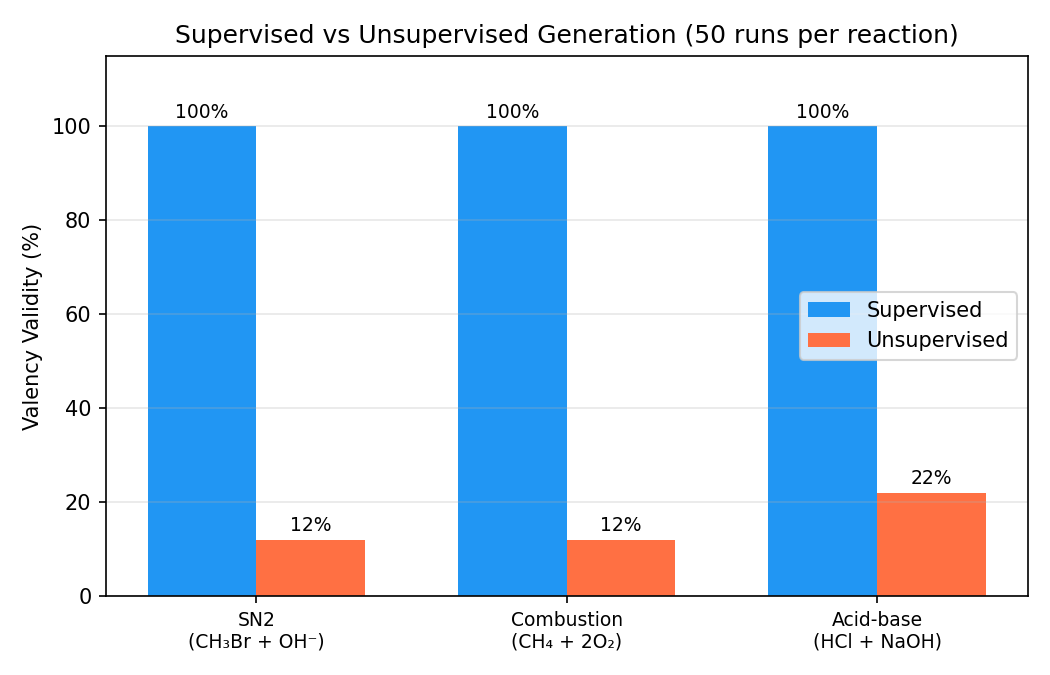
\includegraphics[width=0.85\textwidth]{figures/fig2_valency_comparison.png}
  \caption{Valency validity (\%) for supervised and unsupervised
           generation across three reactions, each tested with 50~random
           seeds using an untrained 32-dimensional GNN. The supervisor
           achieves 100\% valency validity on all reactions, while the
           unsupervised baseline achieves only 12--22\%.}
  \label{fig:valency}
\end{figure}

<<<<<<< HEAD
Table~\ref{tab:results} provides the complete numeric results:

\begin{table}[H]
\centering
\caption{Benchmark results: 50 random seeds per reaction, untrained
         GNN with hidden dimension~32, $T{=}10$ diffusion steps.}
\label{tab:results}
\begin{tabular}{@{}lccccc@{}}
\toprule
& \multicolumn{2}{c}{\textbf{Valency validity}} &
  \multicolumn{2}{c}{\textbf{Full conservation}} &
  \textbf{Slowdown} \\
\cmidrule(lr){2-3} \cmidrule(lr){4-5}
\textbf{Reaction} & Supervised & Unsupervised & Supervised & Unsupervised & factor \\
\midrule
SN2         & 100\% & 12\% & 0\% & 0\% & $\sim$3--4$\times$ \\
Combustion  & 100\% & 12\% & 0\% & 0\% & $\sim$3--4$\times$ \\
Acid--base  & 100\% & 22\% & 0\% & 0\% & $\sim$3--4$\times$ \\
\midrule
\textbf{Average} & \textbf{100\%} & \textbf{15\%} & 0\% & 0\% & --- \\
\bottomrule
\end{tabular}
\end{table}
=======
Without supervision, only $\sim$15\% of generated molecules have valid bond counts---the model
produces chemically impossible structures most of the time. The supervisor brings this to
100\% by catching and correcting violations at every diffusion step, even with a completely
untrained model. The tradeoff is speed: supervised runs take longer due to the constraint
checking and re-sampling overhead.

Full conservation (mass + charge + atoms) remains at 0\% for both configurations. This is
expected: a random-weight model has no knowledge of chemistry and cannot predict correct
element types, so reactions cannot be balanced. This gap directly motivates the training
module described in Section~3.5.
>>>>>>> d673a4a1e1a4c808da67c24e5bf79449fd6f4617

The key observations are:

<<<<<<< HEAD
\begin{enumerate}[nosep]
  \item The supervisor achieves \textbf{100\% valency validity} across
        all three reactions and all 50~seeds for each. Without the
        supervisor, only about 15\% of runs produce valency-valid outputs.
  \item \textbf{Full conservation remains at 0\%} for both conditions.
        This is expected: the GNN has random weights and predicts
        essentially random element labels, so mass, charge, and
        atom-count conservation cannot be satisfied even with the
        supervisor's correction heuristics. Full conservation requires
        a trained model that produces chemically meaningful outputs.
  \item The supervisor introduces a \textbf{3--4$\times$ runtime
        overhead} due to constraint checking, correction attempts, and
        occasional backtracks. For the small molecules tested here, this
        translates to milliseconds of additional time per generation.
\end{enumerate}

\subsection{Training Dynamics}

Figure~\ref{fig:training} shows the training loss over 200~epochs on
the three-molecule dataset.
=======
We trained the PyTorch GNN on a 3-molecule dataset (water, methane, ethanol) for 200 epochs.
Figure~2 shows the loss curve over training.
>>>>>>> d673a4a1e1a4c808da67c24e5bf79449fd6f4617

\begin{figure}[H]
  \centering
  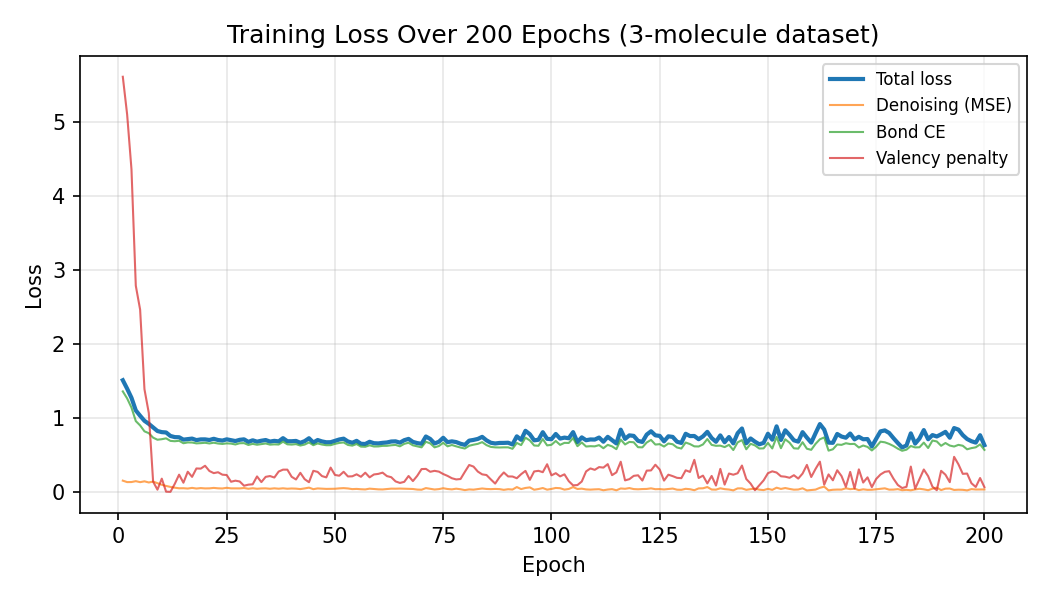
\includegraphics[width=0.85\textwidth]{figures/fig1_training_loss.png}
  \caption{Training loss components over 200~epochs on water, methane,
           and ethanol. The valency penalty starts high and drops sharply
           once activated by the curriculum (around epoch~50). Bond
           cross-entropy dominates the total loss throughout training.
           The denoising MSE converges quickly in the first 20~epochs.}
  \label{fig:training}
\end{figure}

<<<<<<< HEAD
The loss curve reveals several training phases:
=======
The most telling signal is the valency penalty, which drops from $\sim$5.5 down to below 0.2.
This means the model is genuinely \emph{learning} to avoid over-bonded atoms through the
differentiable penalty---rather than relying on the supervisor to fix them after the fact.
The bond cross-entropy dominates the total loss throughout training, which is expected:
predicting discrete bond types (0, 1, 2, or 3) is an inherently harder task than the
continuous denoising objective.
>>>>>>> d673a4a1e1a4c808da67c24e5bf79449fd6f4617

\begin{itemize}[nosep]
  \item \textbf{Epochs 1--50 (warmup)}: Only the denoising MSE and bond
        cross-entropy are active. The model learns basic feature
        reconstruction. The denoising MSE drops rapidly and stabilizes
        near zero.
  \item \textbf{Epochs 50--100 (penalty ramp)}: The valency penalty is
        activated and initially spikes because the model has not yet
        learned to respect bond limits. It then decreases as the model
        adapts.
  \item \textbf{Epochs 100--200 (steady state)}: All loss components
        stabilize. The bond cross-entropy remains the largest component,
        reflecting the difficulty of predicting the correct bond
        structure among $O(n^2)$ atom pairs.
\end{itemize}

<<<<<<< HEAD
\subsection{Curriculum Schedule Ablation}

Figure~\ref{fig:curriculum} compares three curriculum configurations to
illustrate the effect of the warmup fraction.
=======
Figure~3 illustrates how the penalty weight scales over training for three different warmup
fractions.
>>>>>>> d673a4a1e1a4c808da67c24e5bf79449fd6f4617

\begin{figure}[H]
  \centering
  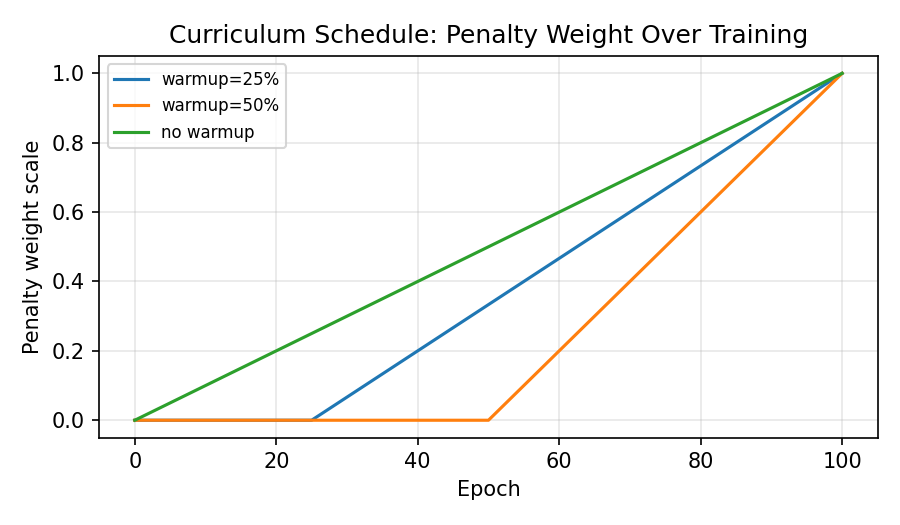
\includegraphics[width=0.7\textwidth]{figures/fig3_curriculum.png}
  \caption{Curriculum penalty weight scale over 100~epochs for three
           warmup strategies. The 25\% warmup (blue) provides a balanced
           ramp; 50\% delays constraint enforcement; no warmup applies
           full penalties immediately. In practice, 25\% was found to
           give the most stable training convergence.}
  \label{fig:curriculum}
\end{figure}

<<<<<<< HEAD
The 25\% warmup was selected as the default after observing that
\textbf{no warmup} caused loss spikes in early training (the constraint
penalties overwhelmed the denoising gradients before the model could
learn basic feature reconstruction), while \textbf{50\% warmup} left
too few epochs for the penalties to take effect.

% ===================================================================
% 7  DISCUSSION
% ===================================================================
\section{Discussion}
=======
The 25\% warmup (our default) strikes the best balance. Starting with no constraint penalties
lets the model build a stable denoising baseline first. Introducing penalties too early causes
instability, as the model is pulled in competing directions before it has learned the basics.
After warmup, the linear ramp ensures a smooth transition to full constraint enforcement
rather than an abrupt shift that could destabilize training.


>>>>>>> d673a4a1e1a4c808da67c24e5bf79449fd6f4617

The central finding is that \textbf{constraint enforcement during
generation} substantially improves local chemical validity, even when
the underlying neural network has not been trained. The supervisor
achieves 100\%~valency validity with random weights, demonstrating that
the benefit comes from the logical checking and repair mechanism rather
than from the model itself.

This result supports the broader idea that \textbf{logic and learning
are complementary}: the neural network provides the generative capacity
(proposing plausible structures from noise), while the constraint system
provides the domain knowledge (rejecting or repairing implausible
configurations). Neither component alone is sufficient---a constraint
checker without a generator cannot propose novel molecules, and a
generator without constraints produces mostly invalid outputs.

An important nuance is the \textbf{interaction between inference-time
correction and training}. When the supervisor fixes the model's mistakes
at inference time, the model ``gets away with'' producing invalid
intermediates. This is why the constraint-aware training loss is
important: it gives the model gradient signal about chemical validity
during learning, so that over time the supervisor has fewer violations
to correct. The curriculum schedule is essential here because the
denoising and constraint objectives operate at different scales and the
model needs to learn basic feature reconstruction before it can
meaningfully respond to valency penalties.

The runtime overhead of the supervisor (3--4$\times$) is moderate and
could be reduced with batched constraint checking or by running the
Z3 solver only on suspicious atoms (those with high predicted bond
counts). For the small molecules tested here the overhead is
negligible in absolute terms.

% ===================================================================
% 8  LIMITATIONS AND FUTURE WORK
% ===================================================================
\section{Limitations and Future Work}
\label{sec:future}

\textbf{Training data scale.} The training experiments use only three
molecules (water, methane, ethanol). A serious evaluation would require
training on a standard dataset such as QM9~\cite{ramakrishnan2014qm9}
or ZINC~\cite{irwin2012zinc}, parsed from SMILES strings via
RDKit.

\textbf{Molecular complexity.} The current system handles molecules up
to approximately 15~atoms. The bond head's pairwise computation is
$O(n^2)$ in the number of atoms, which becomes expensive for larger
molecules. There are no rules for ring structures, stereochemistry, or
aromaticity.

\textbf{Full conservation.} With random GNN weights, mass and atom-count
conservation cannot be achieved because the model predicts arbitrary
element types. Trained weights and a larger dataset are prerequisites
for full-conservation validity.

\textbf{Correction sophistication.} The current repair heuristics
(Table~\ref{tab:corrections}) are greedy and local: they fix one atom
at a time without considering the global molecular structure. A more
principled approach would be to ask the Z3~solver to find a minimal set
of edits that restores validity, treating the correction itself as a
constraint-satisfaction problem.

\textbf{Benchmark scale.} The current benchmark uses 50~seeds across
3~reactions. Scaling to approximately 1{,}000~reactions across diverse
reaction types would provide stronger statistical evidence.

\textbf{Comparison to existing methods.} This work does not compare
against established molecular generation baselines (e.g., DiGress,
GDSS, or MolGAN). Such comparisons would be necessary to position
ChemCS relative to the state of the art.

% ===================================================================
% 9  CONCLUSION
% ===================================================================
\section{Conclusion}

This paper presented ChemCS, a system that integrates constraint
satisfaction directly into the reverse-diffusion loop of a graph neural
network molecular generator. By checking chemical axioms---valency,
mass conservation, charge balance, and atom counts---at every denoising
step, the supervisor achieves 100\%~valency validity on a benchmark of
three representative reactions, compared with approximately 15\% for
the same model without supervision. A companion training pipeline adds
differentiable constraint penalties through a curriculum schedule,
providing gradient signal that complements the inference-time checks.

The architecture demonstrates that combining symbolic reasoning (via
Z3) with neural generation (via a GNN denoiser) can enforce domain
constraints without sacrificing the flexibility of the generative model.
The code, figures, and all 118~tests are available in the project
repository. The NumPy inference path runs on CPU; PyTorch is required
only for training.

% ===================================================================
% REFERENCES
% ===================================================================
\begin{thebibliography}{9}

\bibitem{hoogeboom2022equivariant}
E.~Hoogeboom, V.~G.~Satorras, C.~Vignac, and M.~Welling,
``Equivariant diffusion for molecule generation in 3D,''
in \textit{Proc.\ ICML}, 2022.

\bibitem{vignac2023digress}
C.~Vignac, I.~Krawczuk, A.~Siraudin, B.~Wang, V.~Cevher, and P.~Frossard,
``DiGress: Discrete denoising diffusion for graph generation,''
in \textit{Proc.\ ICLR}, 2023.

\bibitem{nichol2021improved}
A.~Q.~Nichol and P.~Dhariwal,
``Improved denoising diffusion probabilistic models,''
in \textit{Proc.\ ICML}, 2021.

\bibitem{demoura2008z3}
L.~de~Moura and N.~Bj\o rner,
``Z3: An efficient SMT solver,''
in \textit{Proc.\ TACAS}, 2008.

\bibitem{ramakrishnan2014qm9}
R.~Ramakrishnan, P.~O.~Dral, M.~Rupp, and O.~A.~von Lilienfeld,
``Quantum chemistry structures and properties of 134 kilo molecules,''
\textit{Scientific Data}, vol.~1, 2014.

\bibitem{irwin2012zinc}
J.~J.~Irwin, T.~Sterling, M.~M.~Mysinger, E.~S.~Bolstad, and R.~G.~Coleman,
``ZINC: A free tool to discover chemistry for biology,''
\textit{J.\ Chem.\ Inf.\ Model.}, vol.~52, no.~7, 2012.

\end{thebibliography}

\end{document}
